\documentclass[12pt, a4paper]{article}
\usepackage{caption}
\usepackage{graphicx}
\usepackage{svg}
\usepackage{hyperref}
\usepackage{xcolor}
\hypersetup{
colorlinks=false,% hyperlinks will be black
  linkbordercolor=blue,% hyperlink borders will be red
  pdfborderstyle={/S/U/W 1}% border style will be underline of width 1pt
}

\usepackage{listings}
\usepackage{tikz-network}
\usepackage{amsmath, amsfonts, amssymb, amsthm}
\usepackage{algpseudocode}
\usepackage{algorithm}
\title{Algortihms and datastructures}
\date{2022}
\author{Kristoffer Klokker}
\begin{document}
	\maketitle
	\clearpage
	\tableofcontents
	\clearpage
		\section{Algorithm analyse}
			An algorithm must stop for all input and give the correct output.\\
			An algorithms quality is determined from:
			\begin{itemize}
				\item Speed
				\item Memory used
				\item Complexity of implmentation
				\item Other use cases like stability
			\end{itemize}
			\subsection{Algorithm speed}
				The measure speed and memory the worst case of the algorithm is always used due to its simplicity in calculations and gurantee. \\
				The measurement is used as a function of input size using the big O notation, which says for a given input with $n$ size it will take $n^2$  time to run for example.\\
				In reality the speed of an algorithm is not equivalent to the input size due to small constant in every operation but these are so miniscule, they should not be considered. A function may be tuned to have lower constants but this is more a topic for theoretical algorithm optimization.\\
				When comparing algorithm speed the math relations symbols are replaced as such:
				\begin{itemize}
					\item $= -\; \Theta$ Theta
					\item $\leq -\; O$ O
					\item $\geq - \;\Omega$ Omega
					\item $< -\; o$ little o
					\item $> - \;\omega$ little omega
				\end{itemize}
				When comparing the speed of two algorithms the following methods can be used:
				\begin{align*}
					\lim\limits_{n\rightarrow \infty}\frac{f(n)}{g(n)}>&0  &&f(n)=\Theta(g(n))\\
					\lim\limits_{n\rightarrow \infty}\frac{f(n)}{g(n)}=&0  &&f(n)=o(g(n))
				\end{align*}
				The generel speeds of alogirthms in order is:
				$$1,\; \log_2n,\; \sqrt{n},\; n,\; n\log_2n,\; n\sqrt{n},\; n^2,\; n^3,\; n^{10},\; 2^n$$
			\subsection{Ram-model}
				To analyze an algorithm a model is used most often the ram model.
				The ram model is a very simple interpretation of a computer.\\
				The model consist of a CPU, memory and basic operation (add, sub, mult, shift, move, jump)\\
				The time of the algorithm is then measured in amount of basic operations done.\\
				The memory is determined as the amount of memory cell used.
		\section{Sorting algorithms}
			Sorting algorithms are used to sort an array of items in an ascending order.\\
			\subsection{Insertion sort}
				One of the most simple sorting algorithms.\\
				Works by going through the list from index 1 and moves moves every entry before the element 1 up until the element is to the right of an element smaller than the element.\\
				This will therefore have a run time of $O(n^2)$ due to the scenario where the array is in decending order where it will moves $n-1,n-2,..,1$ elements which is $\sum\limits_{j=1}^nj=\frac{(n-1)n}{2}\leq\frac{n^2-n}{2}=n^2$
				\begin{algorithmic}[1]
					\State Insertion-Sort($A,n$)
					\For{$j=1$ to $n$}
						\State $key = A[j]$
						\State $i=j-1$
						\While {$i\geq0$ and $A[i] > key$}
							\State $a[i+1]=A[i]$
							\State $i = i-1$
						\EndWhile
						\State $A[i+1]=key$
					\EndFor
				\end{algorithmic}
			\subsection{Selectionsort}
				Selectionsort is done by taking all elements and then searching for the smallest element and inserting it into the list.\\
				This will result in the same run time $O(n^2)$ due to the same reasoning as insertionsort.\\
				\begin{algorithmic}[1]
					\State Selection-Sort($A,n$)
					\State Array output $= new Array(n)$
					\State $i = 0$
					\While {$i<n$}
						\State $output[i] = A[i]$
						\State $A[i].remove()$
						\State $i++$
					\EndWhile
				\end{algorithmic}
			\subsection{Merge sort}
				Merge sort is an sorting algorithm which is based on the simple merge of two sorted list. Here a new list is created and for every element of the two list, is the lowest value choosen from the first place of the list and putted into the new list. This is is done until both list are empty and when sorting the undefined element is simply equal to infinity when compared.\\[5mm]
				To make this into an sorting algorithm, every element in an unsorted list is made into to list of length 1. Then merge is performed on the lists in pairs of two, from which new sorted lists emerges. This is done until a single lists is left with all the elements which is now sorted. \\[4mm]
				 The speed of this sorting algorithm will therefore be $n\lceil\log_2n\rceil$ due to for every level of merge there will be performed $n$ operations. The amount of levels of merges are equal to $\log_2n$ due to first there will be $n$ lists, then $n/2$ lists, and then $n/2^2$. This will continue until $n/2^k=1$ which rearranged to find $k$ will be $log_2n=k$.\\
				 The ceiling of $\log_2n$ is due to in scenarios where the list length is not a potens of two and a list has no pair in this case it will go on to the next level and thus creating a new level once the list has 1 more item than a potens of two.
				 \begin{figure}
				 	\centering
				 	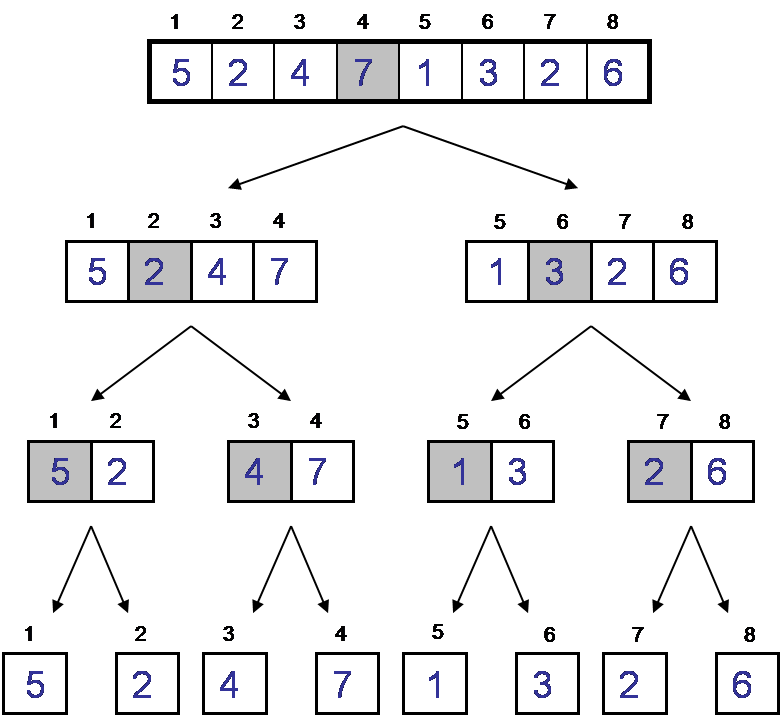
\includegraphics[width=300px]{assets/mergeSort.png}
				 	\caption{Merge sort list split up illustration from j2eereference.com}
				\end{figure}
			\subsection{Quick sort}
				A recursive sorting algorithm which runs mostly at $O(n\log n)$ time but worst case is $O(n^2)$.\\
				The sorting algorithm is smart due to it not needing subarrays copies and working in the original array.\\
				The main idea, is choosing an element in the array, then sorting everything in two baskets lower or equal and higher.\\
				Then the element is placed between the two baskets and quick sort is ran upon the two baskets.
				\begin{algorithmic}[1]
					\State Quick-Sort($A,p,r$)
					\If {$r \leq p$} \State return; \EndIf
					\State $i = p$
					\For {$j=p$ to $r$}
						\If {$A[j] \leq x$}
							\State $temp = A[i]$;
							\State $A[i] = A[j]$;
							\State $A[j] = temp$;
							\State $i=i+1$;
						\EndIf
					\EndFor
					\State $temp = A[i]$;
					\State $A[i] = A[r]$;
					\State $A[r] = temp$;
					\State $Quick-Sort(A,p,i-1)$;
					\State $Quick-Sort(A,i+1,r)$;
				\end{algorithmic}
				The arguments is the array $A$ the start of the sort $p$ and the end $r$.\\
				Here it is seen that in the for loop if the current element is smaller than the choosen element it is switched with the first element in larger basket such that the smaller basket is in front.\\
				In case the element is larger nothing is done. Then at the end the choosen element is switched with the first element of the larger bucket.
			\subsection{Heap sort}
			\label{sec:HeapSort}
				Heap sort is based on the Heap and runs in $O(n\log n)$ and uses no extra space. The heap which is a binary tree which follows heap order. The heap order dictates that a parent should always be greater or equal to its children. \\
				The tree should also have heap shape, which is all branches should be the saem height with a maximum difference of 1. In case of a larger branch it should be on the left side of the tree.\\
				This heap can is illustrated as a tree but is actually an array. Here the arrays first entry is the root, the roots children will then be at index 2 times index and 2 times index + 1\\
				This means the parent is at $\lfloor i/2 \rfloor$ relative to the child.
				\begin{figure}[h!]
					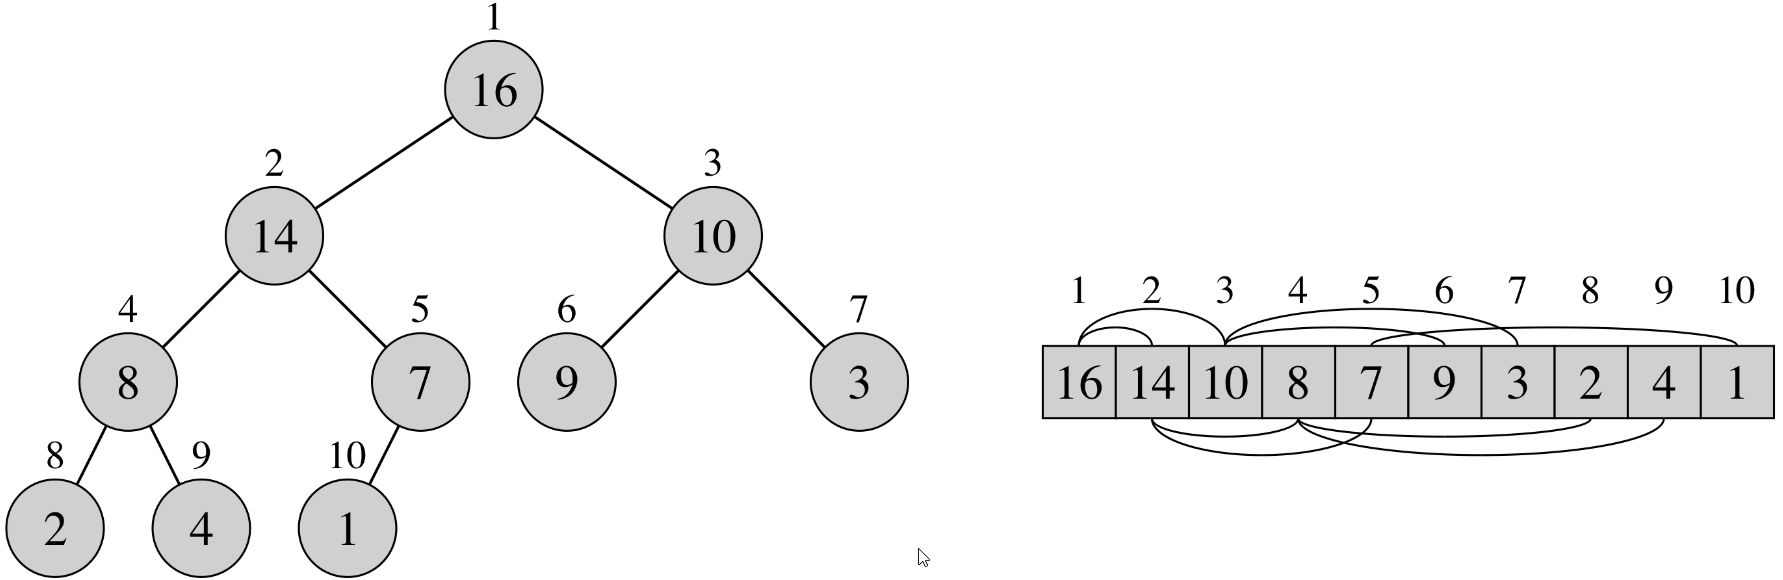
\includegraphics[width=300px]{assets/heapAsArray.png}
					\center
					\caption{The heap illustration and the heap array}
				\end{figure}
				Heap sort then uses the heap array, and when sorting the first entry or the root is switched with the last entry of the heap array.\\
				By this the size of the heap array shrinks with 1 and the rest of the array is the sorted array.\\
				When switched the heap is reconstructed.\\
				The reconstruction process is as follows:
				\label{code:MaxHeapify}
				\begin{algorithmic}[1]
					\State Max-Heapify($A,i,n$)
					\State $l = 2i$;
					\State $r =2i+1$;
					\If {$l\leq n$ and $A[l] > A[i]$}
						\State $largest = l$;
					\Else
						\State $largest = i$;
					\EndIf
					\If {$r \leq n$ and $A[r] > A[largest]$}
						\State $largest = r$;
					\EndIf
					\If {$largest != i$}
						\State $temp = A[i]$;
						\State $A[i] = A[largest]$;
						\State $A[largest] = temp$;
						\State $Max-Heapify(A,largest,n)$;
					\EndIf
				\end{algorithmic}
				The $n$ is used as the length of the heap and $i$ is the current node to check.\\
				The first if check if the left child is larger, the second checks if the right child is larger, and the third check if something should be changed and if then call itself upon the newly changed child.\\
				With this function in mind heap sort becomes: 
				\begin{algorithmic}[1]
					\State HeapSort($A,n$)
						\State Max-Heapify(A,n);
						\For {$i=n$; $2 < i$; $i--$;}
							\State $temp = A[i]$;
							\State $A[i] = A[0]$;
							\State $A[0] = temp$;
							\State Max-Heapify($A,1,i-1$);
						\EndFor
				\end{algorithmic}
				The run time of this is $O(n\log n)$ dut to the trees height will maximally be $\log n$ which will be the number of exhanges $n$ times.
			\subsection{Counter sort}
				Counter sort works in $O(n+k)$ time on arrays of objects represented by integers by having an array with $k$ length. Where $k$ is the highest integer.\\
				It then goes through the orginal array and takes every elements value and uses it as index for the $k$ array and itterate by 1.\\
				Then a new array with length $n$ is made and every element in the $k$ array is added to the new array with the value of elements index as many times as the value of element.
			\subsection{Radix sort}
				Radis sort runs in $O(d(n+k))$ time, where $d$ is amount of digits in largest number and $k$ is the max value of the base of the number system. First Counter sort is done upon every elements lasts digit. Then from the new array counter sort is done again on the second lasts digit. This is repeated as many times as the most digits in the largest number.\\
				This therefore means in the counter sort, the $k$ array only has the length the max value of the number system and instead of itterate it is now a list with references.\\
				This therefore solves the issue of now knowing the largest digit, and the temperary array is a lot shorter.
		\section{algorithms}
			\subsection{Divide-and-Conquer algorithms}
				The same as recursive algorithms.\\
				When illustrated a tree is often used to describe the calls and calls backs\\
				When finding the run time of divide and conquer algorithms, the master theorum is used.\\
				It states:
				$$T(n)=aT(n/b)+f(n)$$
				Where $a$ is the amount of branches created by the algorithm and $b$ is the amount each branch elements is divided by.\\
				$f(n)$ is the run time of the node, for sorting or creating new branches.\\
				It can here be seen that all divide and conquer algorithms fall into 3 categories:
				\begin{itemize}
					\item if $f(n)=O(n^{\log_b(a)-\epsilon})$ then the run time is dominated by the leaves\\
							  and the running time is $T(n)=\Theta(n^{\log_b(a)})$
					\item if $f(n)=\Theta(n^{\log_b(a)})$ then the run time is even on all layers of the tree\\
						and the running time is $T(n)=\Theta(n^{\log_b(a)}\cdot \log(n)$
			 		\item if $f(n)=\Omega(n^{\log_b(a)+\epsilon})$ then the root is the dominating rung time\\
							  and the running time is $T(n)=\Theta(f(n))$
				\end{itemize}
				Where $\epsilon$ is some constant bigger than 0.\\
				Remember: $O - \leq$, $\Theta - =$ and $\Omega - \geq$\\
				If the theorum does not apply, an alternative is writing, a tree with $a$ children at each node, the number of elements in the node $b$ and then then sum up all layers run time.\\[4mm]
				There is instances where to function may fall into two of the cases, for example $T(n)=@T(n/2)+n\log n$.\\
				This case it will fall between case 1 and 2 and can only be found through the tree method.\\
				It shall be noted that, in the case of an uneven divide of the tree, but it does not matter in the runtime since it will only differ with a few constants.
				\subsubsection{Strassen matrix multiplikation}
					Strassen mutliplikation is an algorithm which recursively split up a matrix such the run time get to $O(n^2)$ over the normal calculation method which takes $O(n^3)$\\
					In a given matrix over the size 2x2 the matrix will be divided up in four matrix of each corner. Then strassen discovered a method such only 7 calculation is needed in a 2x2 matrix instead of 8. This therefore makes the problem into a $T(n)=7T(n/2)+n^2$, 7 from the amount of problems, n/2 by the matrix size always halfing and $n^2$ for each  of the 7 problems taking. Therfore makign the runtime $O(n^2)$ using the master theorum.
					The 7 calculation is:
					$\begin{bmatrix}a&b\\ c&d\end{bmatrix}\begin{bmatrix}e&f\\ g&h\end{bmatrix}=\begin{bmatrix}p5+p4-p2+p6&p1+p2\\ p3+p4&p1+p5-p3-p7\end{bmatrix}$
					\begin{itemize}
						\item $p1=a(f-h)$
						\item $p2=(a+b)h$
						\item $p3=(c+d)e$
						\item $p4=d(g-e)$
						\item $p5=(a+d)(e+h)$
						\item $p6=(b-d)(g+h)$
						\item $p7=(a-c)(e+f)$
					\end{itemize}
				\subsubsection{Dynamic programming}
					Dynamic programming is used in recursive algorithms which may have, recalculate a lot of subtasks.\\
					A classic example is fibonacci sequence, where the results are stored in an array, such when f(n)=f(n-1)+f(n-2) is calculated only the first time it is recursively calculated and f(n-2) has already all values in the array.
				\subsubsection{Longest common subsequence}
					To find the longest common subsequence of two string a 2D dyncamic approach can be taken.\\
					The common subsequence is the lenght of the sequence which can be found in both strings.\\
					\begin{figure}[h!]
							  \centering
							  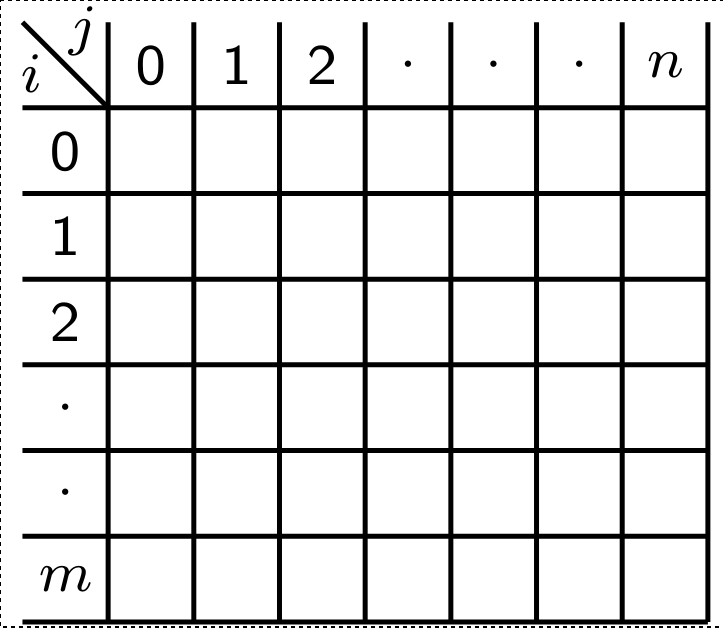
\includegraphics[width=300px]{assets/LCS.png}
							  \caption{A 2D image of finding the longest subsequence}
					\end{figure}
					When finding the sequence it starts and the first character of each string. From here there are 3 cases:
					\begin{itemize}
							  \item They match, so it returns LCS(n.substring(1),m.substring(1))
								\item They do not match, so it returns max(LCS(n.substring(1),m),LCS(n,m.substring(1))
								\item One of the strings are empty, returns 0
					\end{itemize}
					This is illustrated by, the first case an arrow is diagonal, second two arrow to the right and down are created. The last case is at the border where no subsequence is possible.\\
					As seen it will create a path of longest sequence.\\
					The run time is $O(mn)$ and it will also store $mn$ spaces.
			\subsection{Lower bound of comparison sorting algorithms}
				To find the lower bound of comparison sorting algorithms, the comparison model can be used.\\
				The model consist of a binary tree where every branch is a comparison, and the leafs are possible answers.\\
				The run time here is the comparisons, therefore the run time to a leaf is the length of the path. Therefore making worst case height of tree.\\
				It can therefore be seen when sorting an array of $n$ elements there are $n!$  different rearrangement.\\
				Each rearrangement needs a leaf therefore the tree has to have $n!$ leafs.\\
				The maximum amount of leafs in a tree is $2^h$ where $h$ is the height.\\
				Therefore the minimum amount of height will be $2^h\geq n! \rightarrow h\geq \log n!$\\
				\begin{align*}
					h&\geq \log n!\\
					&=\log (n\cdot (n-1)\cdot (n-2)\cdot ...)\\
					&=\log n + \log(n-1) + ...\\
					&\geq \frac{n}{2}\cdot \log(\frac{n}{2})\\
					&=\frac{n}{2}(\log(n)-1)
				\end{align*}		
				It can here be derived via the summation, that $h=\Omega(n\log n)$
			\subsection{Maximum summation of sequential elements in array}
				The most simple version of this, is two pointers with start of seqence and end, where for each element in the array the start is appointed from which all possible ends if summed and the largest value is taken.\\
				This means the algorithm will take $O(n^3)$ due to first every element being appointed as start, from which all elements is tested as the end of sequence, from which the summation is done. This will round up to the worst case being $O(n^3)$\\
				This can be optimized to a run time of $O(n)$, by instead of recalculating everything for every pointer a pointer is started at the start from which an end pointer is also at the start.\\
				Here the largest summation is found, if it is larger than the best sequence it is assigned. Then the end pointer is moved forward and the new element is summed to the recent best sequence. If the sequence summation is now below zero the start pointer is moved to the end otherwise the end pointer is moved forward.
				\begin{algorithmic}[1]
					\State MaxSequence($A$)
					\State $max = 0$
					\State $tempMax = 0$
					\State $i = 0$
					\While {$i<A.length$}
						\State $tempMax = max(tempMax + A[i], 0)$
						\State $max = max(max, tempMax)$
						\State $i++$
					\EndWhile
				\end{algorithmic}
			\subsection{Hashing}
				Hashing is method of getting a idenfiable key to some data.\\
				While the data may have range of indexible data, the hash function is a way to get a smaller index.\\
				The motivation is seen in the following example.\\
				Storing 5 credit card numbers in an array with size of every possible creditcard number would not be optimal.\\
				A simple solution is taking the integer value of the object an using modulo on the desired size of the array.\\
				This will create problems due to some object will collide, as a resolution a list can be created at every index which then can be added.\\
				This will result in slower run time worst case being $O(1)$ for the index and $O(n)$ for finding it in the list.\\
				An alternative is a binary search tree to optimize it to $O(\log n)$.\\
				The ideal hash function will spread out objects as much as possible and a simple an reliable function being
				$$h(k)=((a\cdot k+b) \;mod\; p)\; mod\; m$$
				Where p is a prime larger than the size of the array and a and b are random constant integers $1\leq a \leq p-1$ and $0\leq b \leq p-1$
				\subsubsection{Open addressing}
					An alternative to having a list as hash chain, is using different methods of finding next open position.\\
					The following methods uses a given hash function $h(k,i)$, where $k$ is the given value, and $i$ is the shift.\\
					For every same entry the $i$ variable is increased by 1.\\
					\textbf{Linear hashing}: if the index is taken $i$ is added to index\\
					\textbf{Quadratic hashing}: if the index is taken $i^2$ is added to index\\
					\textbf{Double hashing}: If the index is taken $i\cdot h(k)$ is added.\\
					The reason to use methods which space out index more is to prevent clustering, which can worsen search times.
			\subsection{Greedy algorithm}
				A greedy algorithm is an algorithm which takes the first possible solution. This will always find a local optimum, which may not be global optimal.\\
				The algorithm is based upon taking the problem and taking the best solution at the moment.\\
				To use a greedy algorithm it is important the find and argument for an invariant which holds true such the solution it will find is an optimum.\\[4mm]
				An example to this type of problem is a packing example. The packages have each a weight and a value.\\
				A greedy algorithm will here each package and find it value pr. weight, it then fills up with the most value pr. weight, if there is not enough space it goes to the next package.\\
			\subsection{Bit compression using Huffmans algorithm}
				Huffmans algorithm is a compression algorithm based on shortening bits using frequency.\\
				An example is word shortening, in ASCII a charachter is represented with 8 bits.\\
				But by finding the frequency of each character, the most used characters, can have a shorter bit code.\\
				In order to assign each character a bit code, a tree is made.\\
				Each charchter and its frequency is made as a leaf. Then the two lowest frequency nodes are combined such the two nodes are leafs in a tree where the parent is the combined frequency and the parent is now in upon all nodes.\\
				This is repeated until a true binary tree is made. Then each character is then assigned a bit code by going to the right in the tree will equal to 1 and left equal to 0.\\[4mm]
				This is greedy algorithm which finds the optimum, which can be argued by at first the tree is optimum of two characters.\\
				Then for a the two scenarios where one tree is split such it has a depth of 1+ another tree, it can be seen that, due to the frequency and the single bit in difference, the difference will be constant, therefore neglible. Such that the found tree will always be the optimal tree.\\[4mm]
				The run time will then be $O(n\log n)$ using a heap algorithm and finding frequency is just $O(n)$, so neglible.
		\section{Datastructures}
			\subsection{Priority queues}
				Priority queues are based on the heap structure, which is described in \hyperref[sec:HeapSort]{Heap sort}.\\
				Here the queue objects are given a key from which the value iindicates the priority of the object.\\
				It can here selected if the wanted heap is a max heap or min heap, but most often a max heap.\\
				For the queue to work it uses the following functions:
				\begin{itemize}
					\item Max-Heapify(A,i,n) - makes the array in max heap order with the length $n$ and looks at node $i$
					\item Heap-Extract-Max(A,n) - returns the highest priority object and remove from heap
					\item Heap-Increase-Key(A,i,key) - modifies the key $i$ to a higher value $key$ and place it correctly in heap
					\item Max-Heap-Insert(A,key) - Inserts $key$ into the heap
				\end{itemize}
				\subsubsection{Pseudo code}
					\hyperref[code:MaxHeapify]{Max-Heapify code}
				\begin{algorithmic}[1]
					\State Heap-Extract-Max($A,n$)
					\If {$n < 1$}
						\State error 'Heap underflow'
					\EndIf
					\State $max = A[0]$
					\State $A[0] = A[n-1]$
					\State $Max-Heapify(A,1,n-1)$
					\State return $max$
				\end{algorithmic}
				.\\[3mm]
				\begin{algorithmic}[1]
					\State Heap-Increase-Key($A,i,key$)
					\If {$key < key[i]$}
						\State error 'new key is smaller than current'
					\EndIf
					\While {$i > 0$ AND $A[Parent(i)] < A[i]$}
							\State $temp = A[i]$;
							\State $A[i] = A[i/2]]$;
							\State $A[i/2] = temp$;
							\State $i=i/2$
					\EndWhile
					\end{algorithmic}
				.\\[3mm]
					\begin{algorithmic}[1]
						\State Max-Heap-Insert(A,key,n)
						\State $A.insert(n,-\infty)$
						\State $Heap-Increase-Key(A,n,key)$
					\end{algorithmic}
			\subsection{Binary search tree}
				A binary search tree is a tree which follows inorder.\\
				Inorder states that for a node the left child is smaller and the right child is larger.\\
				By this to get the ordered list a recursive call can be:
				\begin{algorithmic}[1]
					\State list-tree(x)
					\State list-tree(x.left)
					\State print(x)
					\State list-tree(x.right)
				\end{algorithmic}
				This will go through the tree in order, this pseudo code will here print every key, and it should be noded the code does not handle NIL objects.\\
				This operation takes $O(n)$ run time and all other oeparations as mention below will run in $O(height)$. The balanced binary tree will therefore have a height of $\log_2 (n+1) \leq $ height and making the run time $O(\log n)$.
				\subsubsection{Searching a binary tree}
					To search the tree, a comparison is done at each node from which the right child is choosen:
					\begin{algorithmic}[1]
						\State Tree-Search(x,k)
						\If {$x == NIL$ OR $k==key[x]$}
							\State return $x$
						\EndIf
						\If {$k < x.key$}
							\State return $Tree-Search(x.left,k)$
						\Else
							\State return $Tree.search(x.right,k)$
						\EndIf
					\end{algorithmic}
					Find the lowest key, .					
					\begin{algorithmic}[1]
						\State Tree-Minimum(x)
						\While{$x.left != NIL$}
							\State $x = x.left$
						\EndWhile
						\State return $x$
					\end{algorithmic}
					To find the smallest key bigger than key $x$. Works by if right side is not NIL it will be the minumum on the right side otherwise it moves up to the parent until the given node is the left child to the parent.
					\begin{algorithmic}[1]
						\State Tree-Successor($x$)
						\If {$x.right != NIL$}
							\State return Tree-Minimum($x.right$)
						\EndIf
						\State $y=x.parent$
						\While{$y!=NIL$ and $x==y.right$}
							\State x= y
							\State y = y.parent
						\EndWhile
						\State return $y$
					\end{algorithmic}
				\subsubsection{Inserting in the tree}
				\label{sec:BSTInsert}
					\begin{minipage}{0.49\textwidth}
						Tree-Insert(T,z)
						\begin{algorithmic}[1]
							\State $y = NIL$
							\State $x = T.root$
							\While {$x $!=$ NIL$}
								\State $y = x$
								\If {$z.key < x.key$}
									\State $x = x.left$
								\Else
									\State $x = x.right$
								\EndIf
							\EndWhile
							\State $z.p = y$
							\If {$y == NIL$}
								\State $T.root = z$
							\ElsIf {$z.key < y.key$}
								\State $y.left = z$
							\Else
								\State $y.right = z$
							\EndIf								
						\end{algorithmic}
					\end{minipage}
					\begin{minipage}{0.49\textwidth}
						$y$ is the current nodes parent and $x$ is the current node.\\
						Then in the while loop the node is moved down in the correct direction, until it hits NILL.\\
						Then a check is done, if $y$ is NILL the tree is empty and we are at root.\\
						Otherwise the node is placed according to the correct direction to parent.
					\end{minipage}
				\clearpage
				\subsubsection{Deleting a node in the tree}
				When removing an element there is three case according to the number of children equal to NIL:
						\begin{itemize}
							\item 2 - The element is replaced by NIL
							\item 1 - The parent reference is changed to the child
							\item 0 - The succesor to the remove node is inserted instead.
						\end{itemize}
					\begin{minipage}{0.49\textwidth}
						Tree-Delete(T,z)
						\begin{algorithmic}[1]
							\If {$z.left == NIL$}
								\State $Transplant(T,z,z.right)$
							\ElsIf {$z.right == NIL$}
								\State $Transplant(T,z,z.left)$
							\Else
								\State $y=Tree-Min(z.right)$
								\If {$y.p != z$}
									\State $Transplant(T,y,y.right)$
									\State $y.right = z.right$
									\State $y.right.p = y$
								\EndIf
								\State $Transplant(T,z,y)$
								\State $y.left = z.left$
								\State $y.left.p = y$
							\EndIf
						\end{algorithmic}
					\end{minipage}
					\begin{minipage}{0.49\textwidth}
						The delete method uses a $Transplant$ function which arguments are:\\
						 Tree, node1, node2. \\
						Which then switches node1 and node2.\\
						The first if and else if covers the first case and second case with 2 or 1 child equal to NILL\\
						In this case the other child is swapped with the node.\\[4mm]
						The else covers the last case of 0 NILL children.\\
						First the succesor is found by the minimum node of $z$'s right child.\\
						The the if at line 7, checks for if the MIN node is not $z$'s right child.\\
						 If not then the min node $y$ is rotated up as the root of $z$'s right branch, with its parent as right child and the parent left child being $y$s right child.\\
						 Then $y$ substitutes $z$ and takes $z$ left child aswell.\\
						 
					\end{minipage}
				
					
			\subsection{Balanced binary tree}
				The idea behind a balanced binary tree, is a node has another bit representing a color red or black.\\
				The rule is then:
				\begin{itemize}
					\item The root has to be black
					\item A red notes child can not be red
					\item Leafs has to be black
				\end{itemize}
				The rules ensures that the roots childrens height will atmost be different by a factor by 2.\\
				This is due to one branch being all black and the other being red and black all the way.\\
				The implementation of a balanced tree will not be slower due to all the manipulations still running at constant time $O(1)$.
				\subsubsection{Rotation of node}
					Rotations are a needed operation on a node in order to insert and remove nodes, and still uphold balance.\\
					\begin{figure}[h!]
						\center
						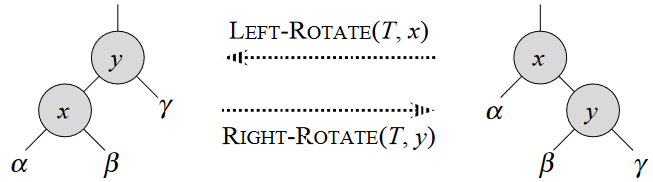
\includegraphics[width=300px]{assets/rotation.png}
						\caption{Illustration of rotation}
					\end{figure}
					
					\begin{minipage}{0.49\textwidth}
						Left-Rotate(T,x)
						\begin{algorithmic}[1]
							\State y = x.right
							\State x.right = y.left
							\If {y.left != T.nil}
								\State y.left.p =x
							\EndIf
							\State y.p = x.p
							\If {x.p == T.nil}
								\State T.root =y
							\ElsIf {x ==x.p.left}
								\State x.p.left = y
							\Else 
								\State x.p.right = y
							\EndIf
							\State y.left = x
							\State x.p = y
						\end{algorithmic}
					\end{minipage}
					\begin{minipage}{0.49\textwidth}
						First y is established and $\beta$ is moved at line 2.\\
						The if at line 3 changes the y left parent reference to x if not nil\\
						The if at line 7 set y as root if x is root\\
						The if at 9 and 11 sets x parents reference to x to y according to direction.
						It can also be seen the rotation will keep inorder due to:
						$$\alpha \leq x \leq \beta \leq  y \leq \gamma$$
						Which is followed both before and after rotation.
					\end{minipage}
			\subsubsection{Insertion in tree}
				First the new element is inserted per usual \hyperref[sec:BSTInsert]{inserting in a binary search tree} as a red node.
				After this rebalancing may be needed, from which four sceanrios are possible:
				\begin{enumerate}
					\item z = root
					\item z.uncle = red
					\item z.uncle = black (trangle)
					\item z.uncle = black (line)
				\end{enumerate}
				\begin{figure}[h!]
					\center
					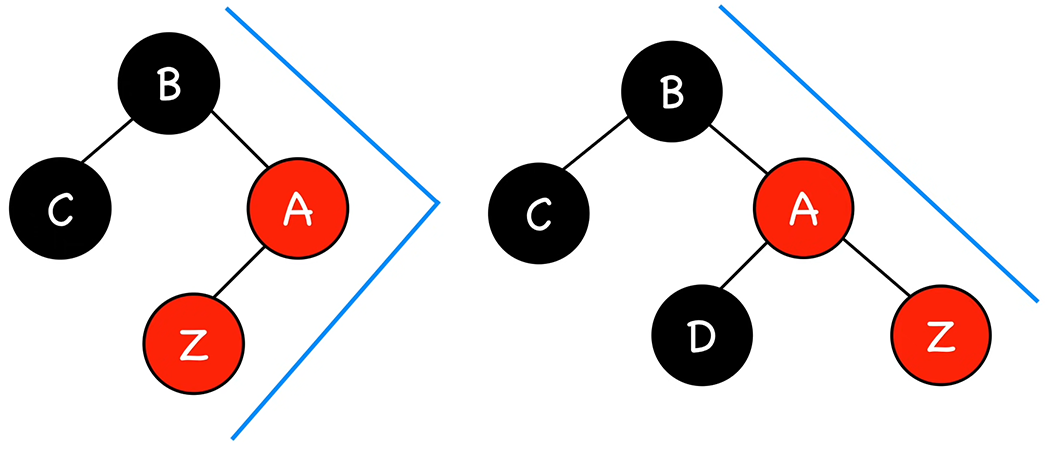
\includegraphics[width=300px]{assets/blackRedTreeTriangeLine.png}
					\caption{A triange shape on left and line shape on right.}
				\end{figure}
				1.\\
				The nodes color should be switched to black\\
				2.\\
				Parent, uncle and grandparent change color\\
				3.\\
				Rotate z.parent in opposite direction of z\\
				4.\\
				Recolor parent and grandparent an rotate z.granparent in oppsite direction of z\\
				RB-Insert-Fix(T,z)
				\begin{algorithmic}[1]
					\While {$z.p.color == red$}
						\If {$z.p == z.p.p.left$}
							\State $y = z.p.p.right$\
							\If {$y.color == red$}
								\State $z.p.color = BLACK$
								\State $y.color = BLACK$
								\State $z.p.p.color = RED$
								\State $z = z.p.p$
							\Else
								\If {$z == z.p.right$}
									\State $z = z.p$
									\State $Left-Rotate(T,z)$
								\EndIf
								\State $z.p.color = BLACK$
								\State $z.p.p.color = RED$
								\State $Right-Rotate(T,z.p.p)$
							\EndIf
						\Else
							\State line 3 - 15 but with left instead of right
						\EndIf
					\EndWhile	
					\State $T.root.color = BLACK$
				\end{algorithmic}
				The while loop runs until, the parent node is not red.\\
				The first check is if the current branch is to the grandparents left.\\
				Then the uncle $y$ is defined.\\
				Then the uncles color is checked. If red then color changes according to case 2.\\
				If black, then if the triangle shape in case 3 is present the rotation is done. From which case 4 will accour and recolor and rotation is done.
			\subsubsection{deletetion in tree}
				First a deletion is done, as normal. The only difference is a fixup function is called if the removed node is black or the successor node was black.\\
				This due to a black therefore being removed or recolored and therefore the black length is not equal on both sides of root.\\
				The fixup function has 4 cases which has to be fixed.
				\begin{enumerate}
					\item red sibling
					\item black sibling with 2 black children
					\item black sibling and nearest child is red and furthest is black
					\item black sibling and the furthest child is red
				\end{enumerate}
				The special child is x and its sibling is w\\
				1. the parent and $w$ changes color and left rotation on parent\\
				2. $w$ changes color to red, $x$ pointer is parent and parent is red\\
				3. $w$ and its red child $\gamma$ changes color and right rotation is performed on $\gamma$\\
				4. $w$ changes color to $x$'s parent, which changes color to black aswell $w$ right child. Left rotation on $x$'s parent\\
				RB-Delete-Fix(T,x)
				\begin{algorithmic}[1]
					\While {$x != T.root$ and $x.color == BLACK$}
						\If {$x== x.p.left$}
							\State $w = x.p.right$
							\If {$w.color == RED$}
								\State $w.color = BLACK$
								\State $x.p.color = RED$
								\State $Left-Rotate(T,x.p)$
								\State $w = x.p.right $
							\EndIf
							\If {$w.left.color == BLACK$ and $w.right.color == BLACK$}
								\State $w.color = RED$
								\State $x = x.p$
							\Else
								\If {$w.right.color == BLACK$}
									\State $w.left.color = BLACK$
									\State $w.color = RED$
									\State $Right-Rotate(T,w)$
									\State $w = x.p.right$
								\EndIf
								\State $w.color = x.p.color$
								\State $x.p.color = BLACK$
								\State $w.right.color = BLACK$
								\State $Left-Rotate(T,x.p)$
								\State $x = T.root$
							\EndIf
						\Else
							\State line 3 - 25 with right and left exhanged
						\EndIf
					\EndWhile
					\State $x.color = BLACK$
				\end{algorithmic}
				
				The code consist of a while loop which only terminates when x is root or x is black.\\
				This is due to if x is the root the color can be changed to black and it will have the same black length on both branches.\\
				The while loop states by checking if the current working branch is to the parents left.\\
				Then the first if covers case 1, and the sibling pointer moves up to $x$'s uncle.\\
				The second if covers case 2, notice here it is guranteed due to the first case that the sibling is black.\\
				The else covers case 3 and 4, where 3 is in the inner if. \\
				It can here be seen that 1 can lead up to all cases, 2 does not lead up to 3 or 4 and 3 always leads up to 4.
		\subsection{Extra data in trees}
			When working with trees, extra information can be stored, such as amount of children in a node.\\
			Saving the amount of children will help deduct the position of the node in a tree walk.\\
			This kind of tree is called an order-statistic tree.\\
			This can be done as seen here, where select returns the node at index $i$ in the walk, and rank returns the nodes index in the walk.\\[4mm]
			\begin{minipage}{0.49\textwidth}
				OS-Select($x$,$i$)
				\begin{algorithmic}[1]
					\State r = x.left.children+1\\
					\If{$i==r$}
						\State return $x$
					\ElsIf{$i<r$}
						\State return $OS-Select(x.left,i)$
					\Else
						\State return $OS-Select(x.right,i-r)$

					\EndIf
				\end{algorithmic}
			\end{minipage}
			\begin{minipage}{0.49\textwidth}
				OS-Rank($T$,$x$)
				\begin{algorithmic}[1]
					\State $r = x.left.children+1$
					\State $y = x$
					\While{$y\neq T.root$}
						\If{$y==y.parent.right$}
							\State $r = r + y.parent.left.children+1$
						\EndIf
						\State $y = y.parent$
					\EndWhile
					\State return $r$
				\end{algorithmic}
			\end{minipage}
			When updating the tree, it is just required to recursively from the button update the affected parents.
					
						\subsection{Disjoint sets}
			Disjoint sets being small partitions of a set.\\
			There are different ways of representing this in a datastructure.\\
			The core of the datastructures are:
			\begin{itemize}
				\item Create a new set
				\item Join two sets
				\item Find set
			\end{itemize}
			\subsubsection{Linked list representation}
				A linked list may be used for the dijoint set. Find set will be constant time and return header of linked list.\\
				Make set also be constant creating a new linked list.\\
				Union must be $n$ time due to one lists reference the header must be changed and other list last node must be linked furhter.\\
				Weighted-union heuristic is a union where the lower lsit is added to the larger list.\\
				Path compression refers to all object in a branch is moved up to be only a depth of 1.\\
				Thus for a making a set of $n$ objects, the run time will be $O(m+n\log n)$, this is due to$\log n$ comes from joining, but since it is done with two sets of same size, the total size will double. Therefore it is only required to perform $\log n$ joins, which is done $n$ times. The $m$ is the amount of find set operations, which is each done in constant time and therefore the total is $m$ time.\\[4mm]
			\subsubsection{Tree representation}
				Another alternative is a tree, where a object in node is representative and root. Find will therefore travel up the tree until found root, make will make its own root, union takes the tree with biggest height as root and make the joining child of the root.\\
				The make set of $n$ and its union and find set will therefore be almost linear with a run time of $O(n+m)$ with $m$ being a slow growing function.\\
				Union by rank refers to making the union tree the optimal height, such when two trees are unioned, the larger tree becomes root such the height is the same, if the same height one is choosen and the height is added by 1.\\
				Path compression is done on find operations. When root is searched for every nodes in the path to find root parent will be set to root, in constant time. Such the height of the tree wil lbe 1.
	\section{Graph}
		Naming conventions:
		\begin{itemize}
			\item Oriented graph - directed graph
			\item Unoriented graph - non directed
			\item Weighted graph - edges has a value
			\item $V$ the set of all vertices
			\item $E$ the set of all edges
			\item $n=|V|$,$m=|E|$
			\item $0\leq m\leq n^2$ for oriented and $0\leq m \leq n^2/2$ for unoriented graph
		\end{itemize}
		\subsection{Representation}
			Graph may be setup as a graph.\\
			List may also be used for each node containing connected vertices.\\
			A matrix can also be used with size $n^2$ if $n_1$ and $n_3$ are connected a 1 is at $n_1,n_3$ and also $n_3,n_1$ .\\
			Therefore in theory the actual size is $n^2/2$ due to it being reflective in an unoriented graph and oriented needs the $n^2$ due to it not being reflective.\\
			Wheras the list version need $O(n+m)$ space
		\subsection{Graph traversal}
			To create a traversal a color coding is used on the vertices.
			\begin{itemize}
				\item white - no edges are used
				\item grey - some edges are used
				\item black - all edges are used
			\end{itemize}
			At the basic the traversal is done by:
			\begin{algorithmic}[1]
				\State GenericGraphTraversal(s)
				\State s.color = grey
				\While{There exists grey vertices}
					\State v = grey vertice
					\If{All edges in v are used}
						\State v.color = black
					\Else 
						\State Choose an unused edge in v, u
						\If {u.color == white}
							\State u.color = grey
						\EndIf
					\EndIf
				\EndWhile
				
			\end{algorithmic}
			Once the algorithm is done all black nodes is connected to $S$ and all white nodes are not.\\
			For finding edges there are different algorithms such as:
			\begin{itemize}
				\item Breadth-First-Search
				\item Depth-First-Search
				\item Priority-Search
			\end{itemize}
			In some cases it may be needed to save for each which node discovered it.\\
			With this info a tree may be made from each node or leaf to root will exist the opposite path in the graph.\\
			\subsubsection{Breadth first traversal}
				This algorithm, start at a vertice, uses all possible edges and then goes to the next vertice.\\
				This algorithm is therefore presented in a queue format.\\
				The idea is all vertices are white and have a distance of infinity.\\
				Then at a vertice the distance is 0, then all vertices directly connected are greyed and gets a distance +1.\\
				Also the added by variable is added.\\
				Then each vertice is added to the queue and everything is ran until the queue is empty.\\
				This will result in every node has the shortest distance, due to essencially every node being taken in order of distance to root and therefore once a node is reached it is the shortest distance.\\
			\subsubsection{Depth first traversal}
				This method is a recursive method, and therefore is refered to using the stack.\\
				The method works by every node is white, and the one choosen is made grey.\\
				A recursive function is then called on a connected node, which makes it grey and call the recursive function on all connected nodes.\\
				By this every connected node will be found recursively. This is seen in the stack by when a node is called it is added to the stack and becomes grey, once every connected node is found and popped of the stack it returns to the grey node and it becomes black and pops off.\\
				Instead of measuring distance a time variable is made, this time variable is added once a node is discovered and once the node turns black.\\
				At both the start and the end of the node the time is saved, such given two nodes (v,u) there relation can be described through their time:
				\begin{itemize}
					\item v and u tims are disjoint and they are note related
					\item v's time interval container u times interval and v is some form of parent to u
					\item the last scenario but flipped around
				\end{itemize}
				The time interval is often written as $s/e$ where $s$ is the start and $e$ is end time\\
				When doing the traversal there are 4 different types of edges which may be classified:
				\begin{itemize}
					\item Tree edge - The most common edge from parent to undiscovered child
					\item Back edge - Edge from child to an anchestor  
					\item Forward edge - Edge from anchestor to some form of existing child
					\item Cross edge - The rest of the edges, mainly edges between branches
				\end{itemize}
				In non oriented graph only tree and back edges exists.\\[4mm]
				Sorting may also be done, if there does not exist any back edges.\\
				No back edges will result in no cycles, and when each vertic is done it can be added to a list.\\
				This will result in every vertice will only point to the right and be in topological order.
		\subsection{Strongly connected compoenents}
			To find strongly connected components Kosarajus algorithm can be used.\\
			The algorithm start be doing a DFS on the graph. Once a node is turned black it is added to a second stack. The order should be decreasing in $u.f$ for each vertex $u$\\
			Then the graphs directions are reversed.\\
			Again DSF is performed, and starts at the end of the second stack. Once the selected stack element is popped off all the traversed nodes is strongly connected.\\
			All other traversed notes in the strongly connected may be also popped of the second stack.\\
			This is done until the second stack is empty.\\
			When reversing the graph all connected components will stay the same due to the SCC's be definition are cycles and can get all around. Whereas the connecting edges between SCC's are cross edges, and by reversing them it is seen that before connected components no longer are connected therefore splitting the connected components.\\
			The reasoning for the reverse topological order, is due to in the topological order, SCC's will be found last, due to them not being connected to the first choosen node.\\
			Therefore be reversing it the strongly conncected components are found earlier and fewer nodes are checked.\\
			This result in the running time being $O(|n|+|e|)$
		\subsection{MST}
			A minimal spanning tree (MST) is a tree which visits every node in a weighted graph, at minimal cose.\\
			This will form a tree and therefore can not contain any cycles.\\
			\subsubsection{Prim Jarnik}
				This is a greedy algorithm, which work with a queue.\\
				A node is then choosen from which all edges is added to the queue.\\
				The minimum is then choosen and used in the tree, which all edges from to not used nodes are inserted to the queue.\\
				The last step is then repeated until the queue is empty, and when meeting a dead edge it is discarded.\\
				This will result in a MST if the graph is all connected, due to the invariant being always choosing the best edge until all edges are evaluated, therefore all edges will be checked.
			\subsubsection{Kruskal}
				Kruskal works by, taking all edges, sorting them in order weight increasing, and then adding all edges which, connects two otherwise unconnected edges.\\
				This can be done by sets in the following algorithm:
				\begin{algorithmic}[1]
					\State A = Ø
					\For{$v\in G.V$}
						\State $Make-Set(v)$
					\EndFor
					\State Sort sets in weight 
					\For{$(u,v)$ from sorted list}
						\If{$Find-Set(u)\neq Find-Set(v)$}
							\State $A=A\cup \{(u,v)\}$
							\State $Union(u,v)$
						\EndIf
					\EndFor
					\State return $A$
				\end{algorithmic}
				This will work by same argument as Prim Jarnik, but this will gurantee a better MST, in case of a bad start for Prim Jarnik.
			\subsubsection{Relax}
				Relax is a method which, simply works by a handler, which goes through every edge and sends it to the relax method.\\
				This method simply handles a new edge and compare to an already known lightest weight. This weight the lightest is saved.
			\subsubsection{Dijkstras}
				This method is a more sophisticated version of relax. Instead of just trying every edge, a start edge is selected. Then every edge from the start node is added to a minimum queue. Then a loop is done until the queue is empty.\\
				The minumum edge in weight is choosen and the receiving nodes edges is added to the queue and called relax upon.\\
				Every used node is saved, such if an edge from the queue is choosen towards an already checked node, the edge is dumped.\\
			\subsubsection{Bellman ford}
				Bellman ford is a tool to check if a graph has a negative loop such a MST is not existing.\\
				The tool simply works by using relax to get the MST, and then for every edge tries to see if adding it will result in a lower weight. Therefore if that exist a negative loop in the graph it will return true.
						
				
			
				
	
				
\end{document}
